\subsubsection*{Show users \faUsers}

Der Administrator erhält zur Benutzerverwaltung, wie in Abbildung~\vref{fig:AdminShowUsersImplement} dargestellt, eine Übersicht über alle im System vorhandenen Benutzer.
Zur erleichterten Suche von Benutzern wurde eine Suchleiste in der Übersicht hinzugefügt.
Diese ermöglicht das Suchen von Benutzernamen oder das Auswählen des Benutzers über ein Dropdown-Menü.
Darüber hinaus erfährt der Administrator den aktuellen Status der in der Anwendung befindlichen Benutzer, wie etwa den Administratorenstatus.

\begin{figure}[H]
	\centering
	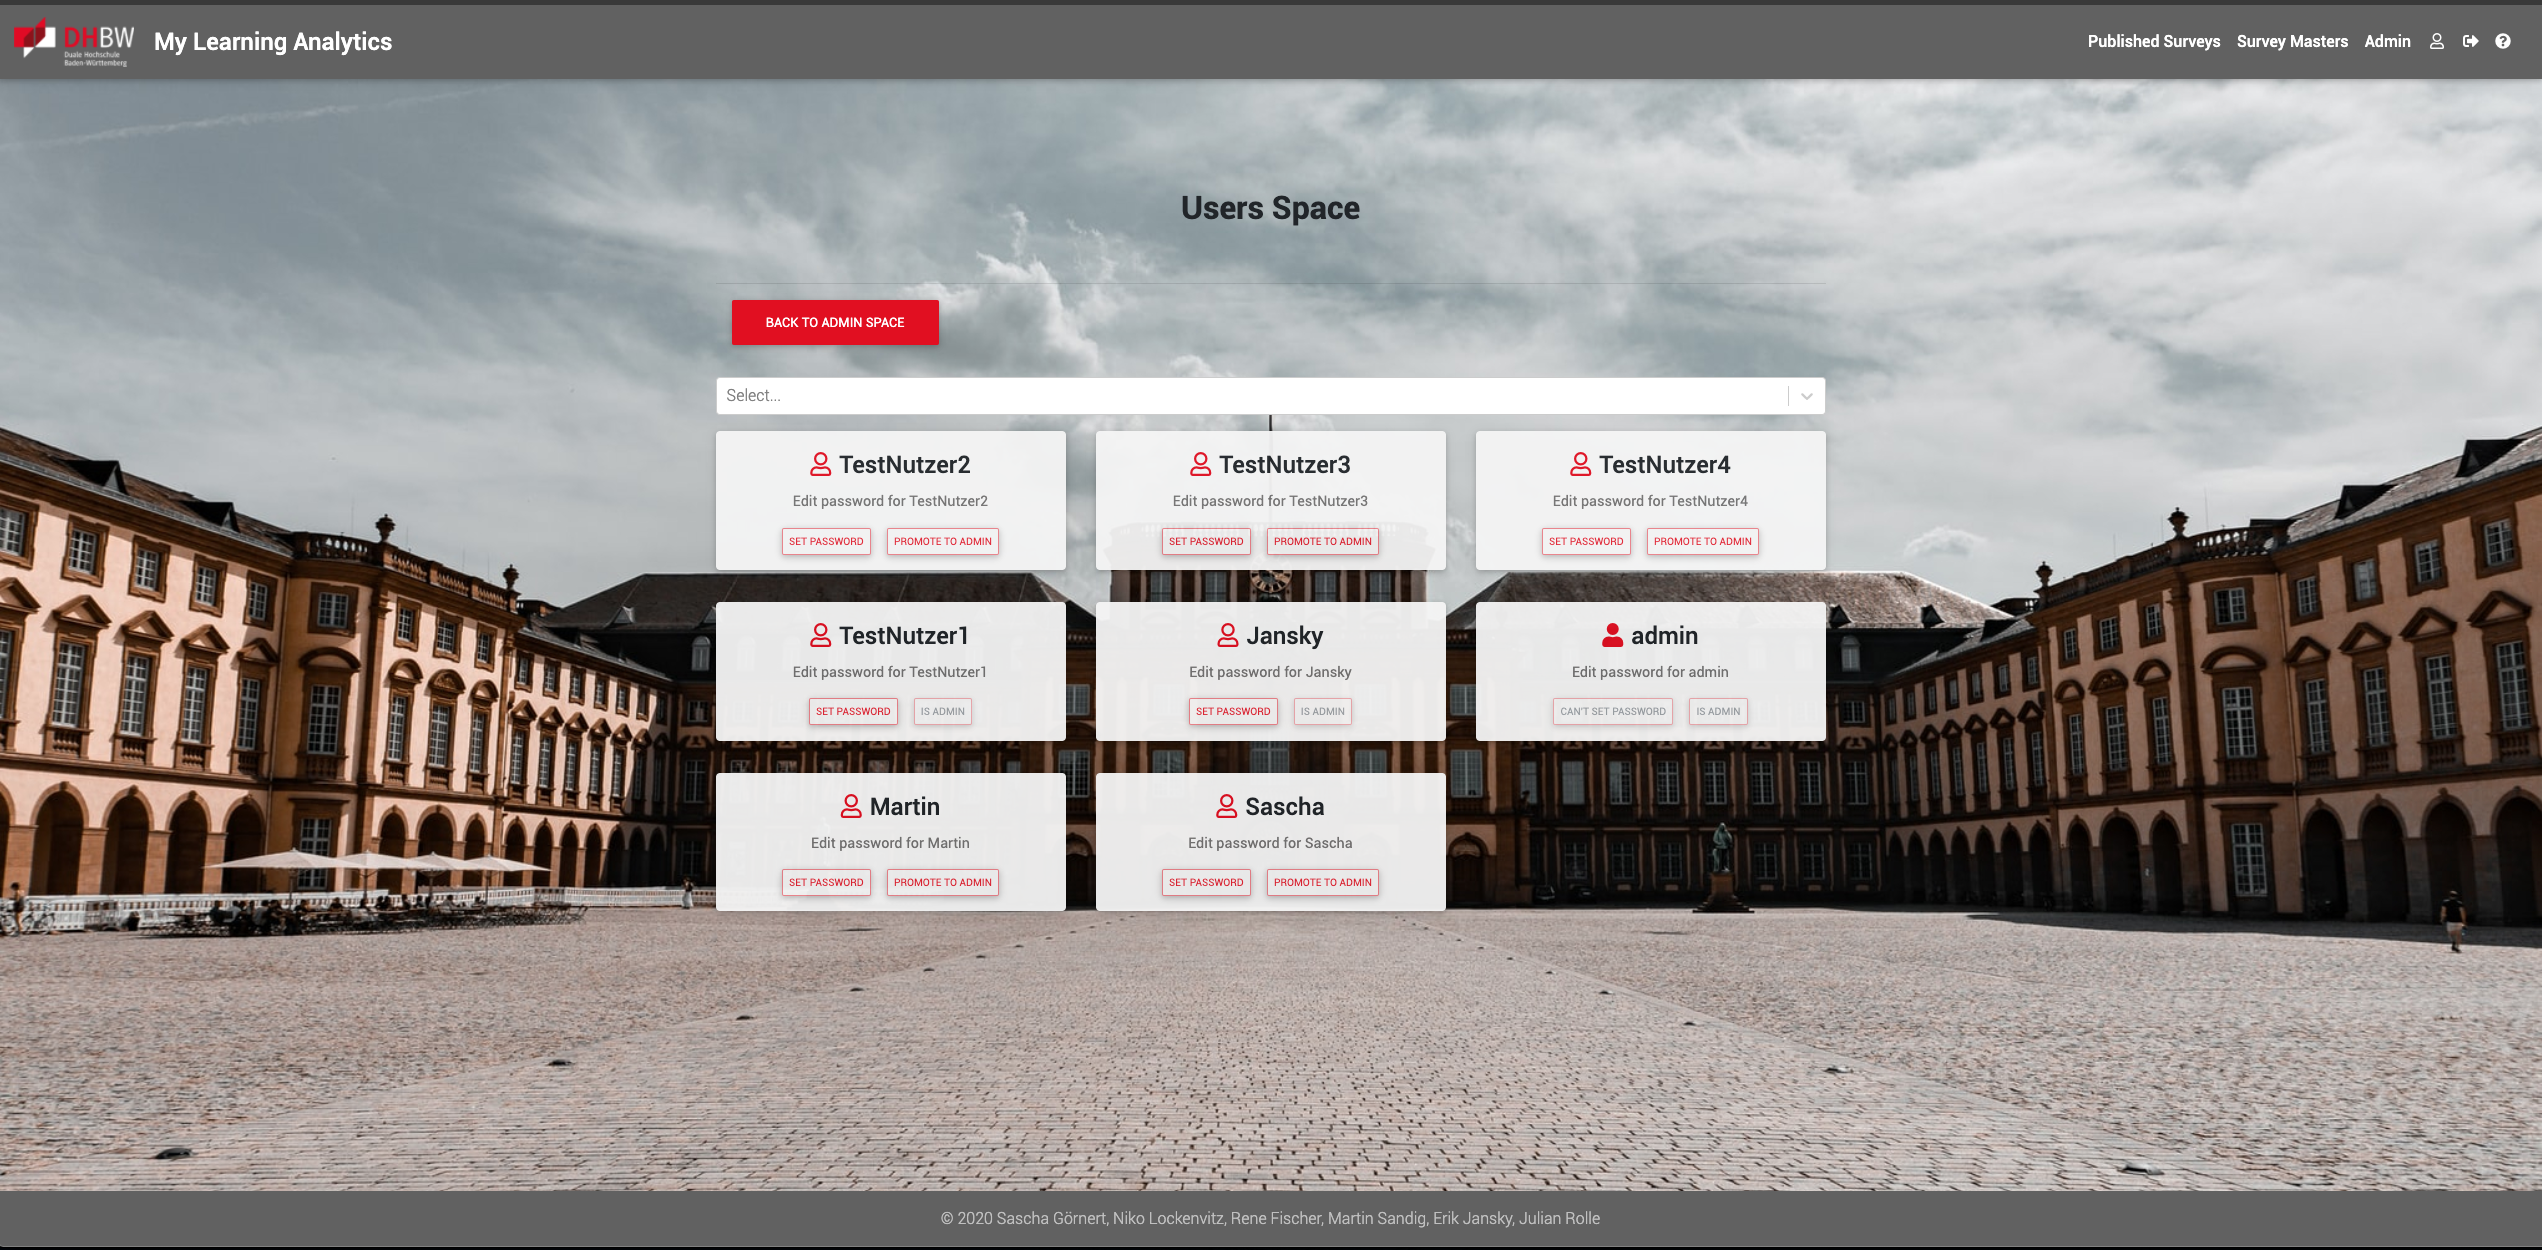
\includegraphics[width=0.95\textwidth, keepaspectratio]{img/client/AdminShowUsers.png}
	\captionsetup{justification=centering, format=plain}
	\caption[\acl{UI}: Benutzerübersicht]{\acl{UI}: Benutzerübersicht \\ \quelleScreenshot}
	\label{fig:AdminShowUsersImplement}
\end{figure}

Der eigene Nutzer wird dabei besonders als \faUser\xspace hervorgehoben, wohingegen andere Benutzer lediglich durch das Icon \faUser[regular]\xspace (Silhouette) dargestellt werden. \newline
Zudem wurde hier das Zurücksetzen des Passworts des Benutzers implementiert, da Benutzer ihr Passwort regelmäßig vergessen.\autocite[Vgl.][]{statistaPasswortVergessen}
Dadurch wird Anforderung~\hyperref[Anf:A6]{A6}, die Pflicht zur Passwortänderung bei zurückgesetztem Passwort, umgesetzt.
Abbildung~\vref{fig:AdminSetNewPasswordImplement} stellt das Zurücksetzen des Passworts über ein Pop-up dar.

\begin{figure}[!htb]
	\centering
	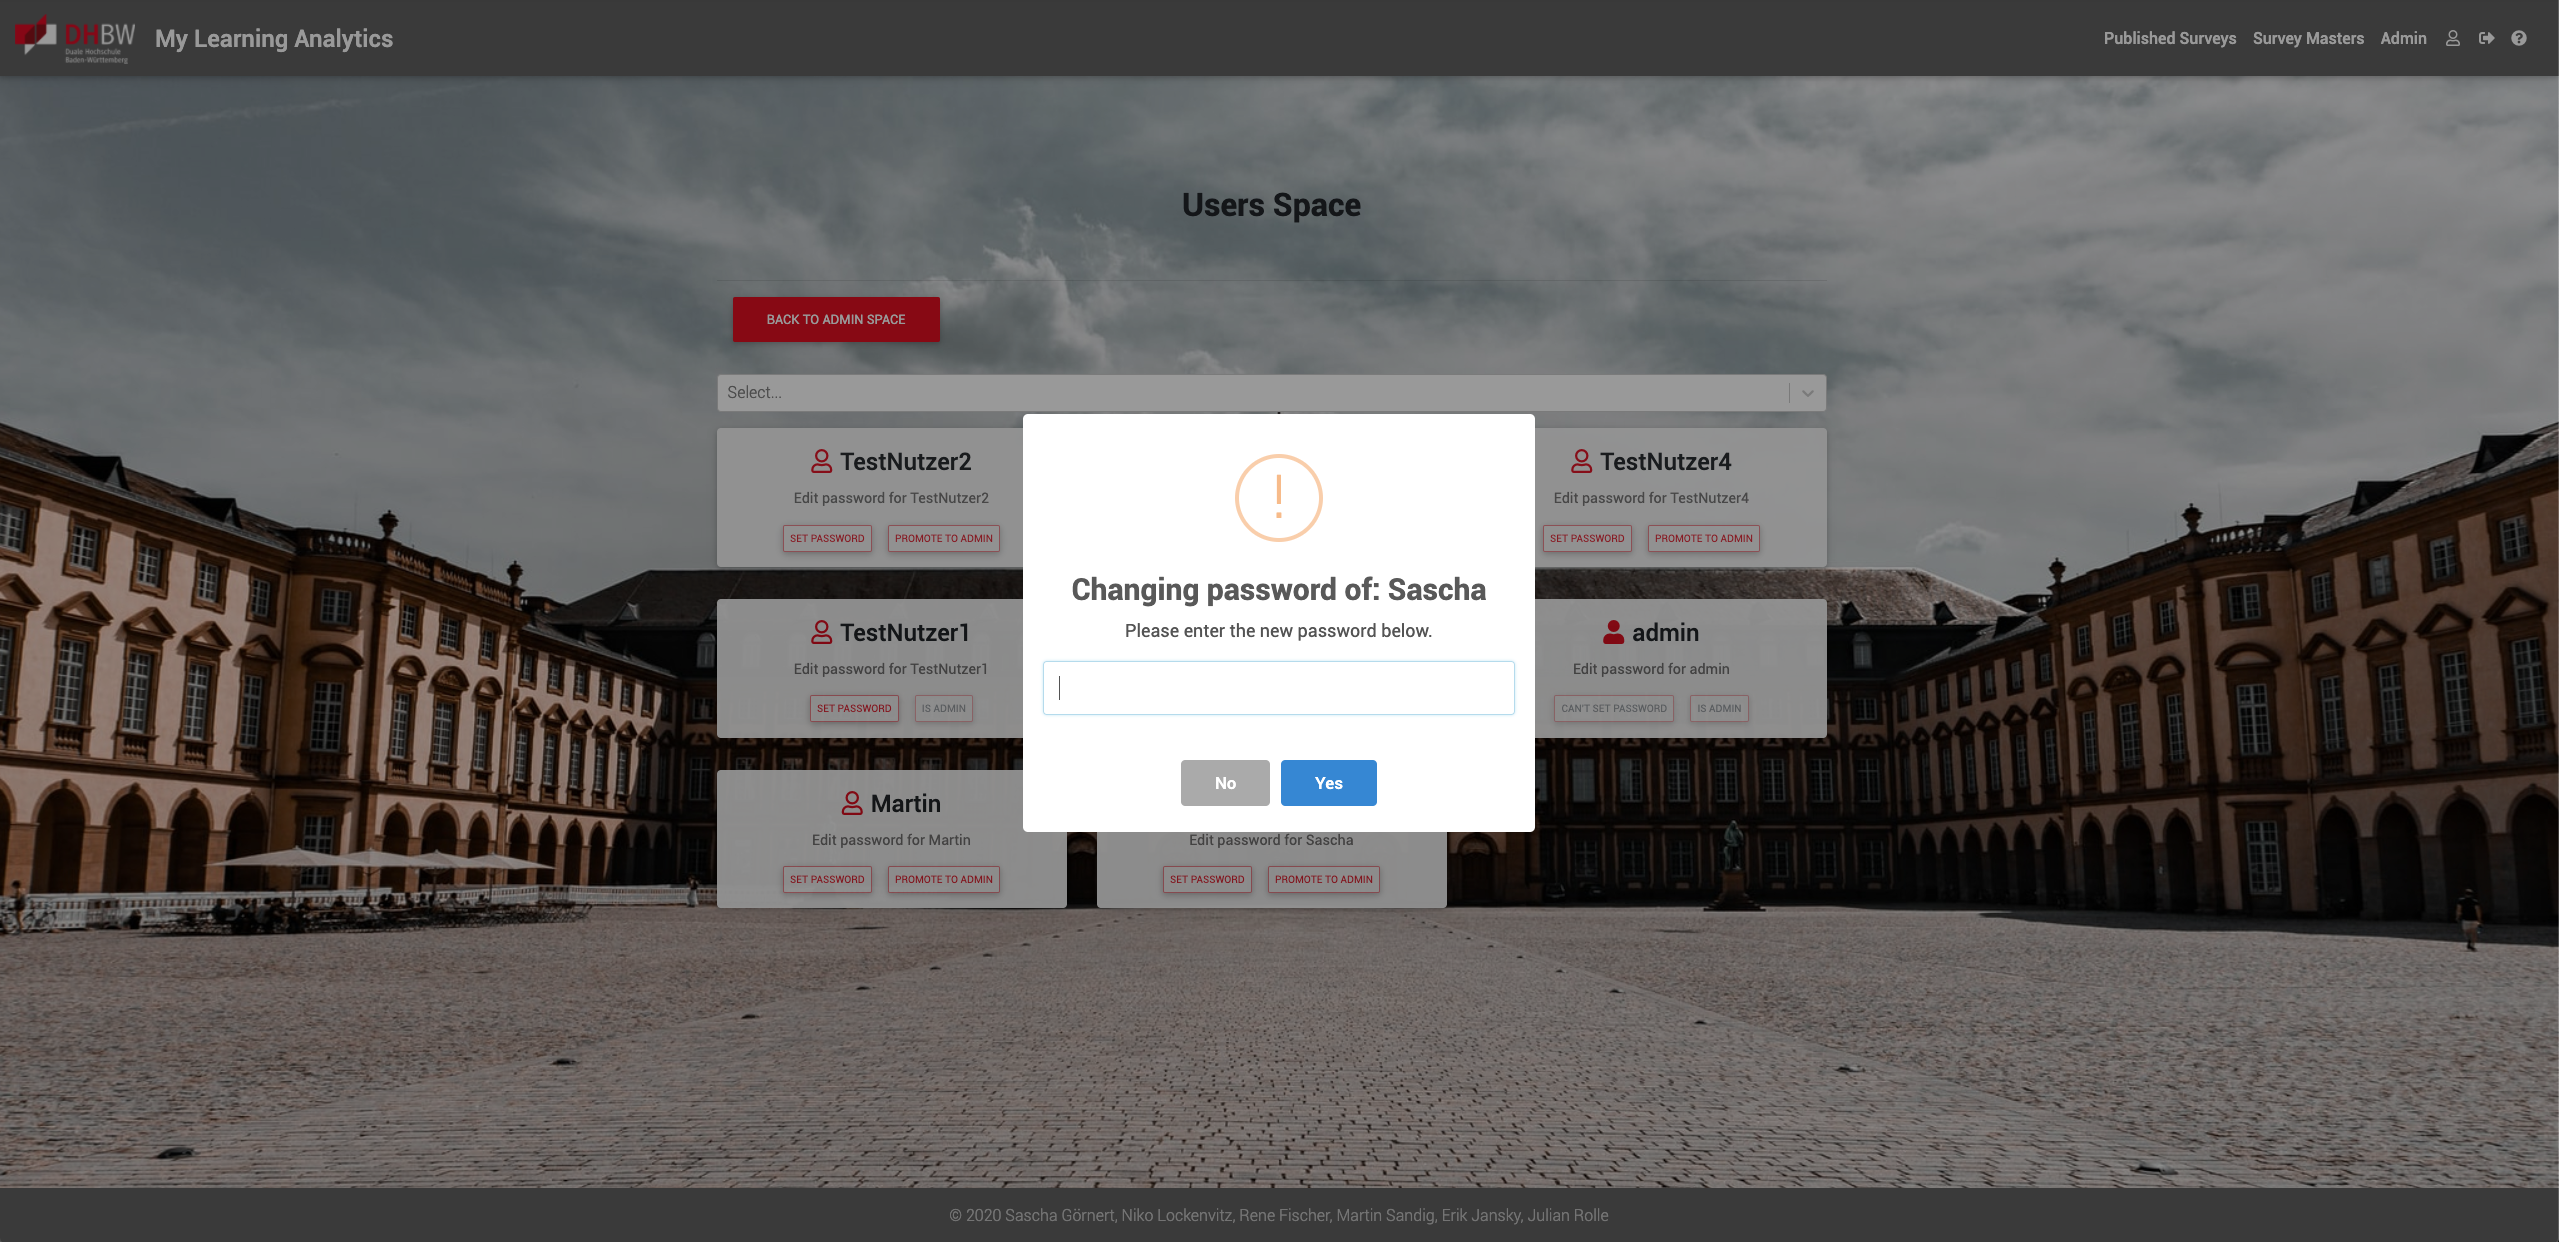
\includegraphics[width=0.95\textwidth, keepaspectratio]{img/client/AdmiSetPasswordOfUser.png}
	\captionsetup{justification=centering, format=plain}
	\caption[\acl{UI}: Zurücksetzen des Passworts]{\acl{UI}: Zurücksetzen des Passworts \\ \quelleScreenshot}
	\label{fig:AdminSetNewPasswordImplement}
\end{figure}

Ein weiteres Feature der Anwendung ist das Ernennen von Administratoren.
Dies geschieht über den Knopf \jinline|Promote To Admin|, welcher in Abbildung~\vref{fig:AdminPromoteToAdminImplement} dargestellt ist.
Zusätzlich dazu muss der Nutzer diese Beförderung über einen weiteren Dialog bestätigen, um Fehler zu vermeiden.
Visuell werden Administratoren hervorgehoben, da der Knopf \jinline|Promote To Admin| durch \jinline|Is Admin| ersetzt wird.

\begin{figure}[!htb]
	\centering
	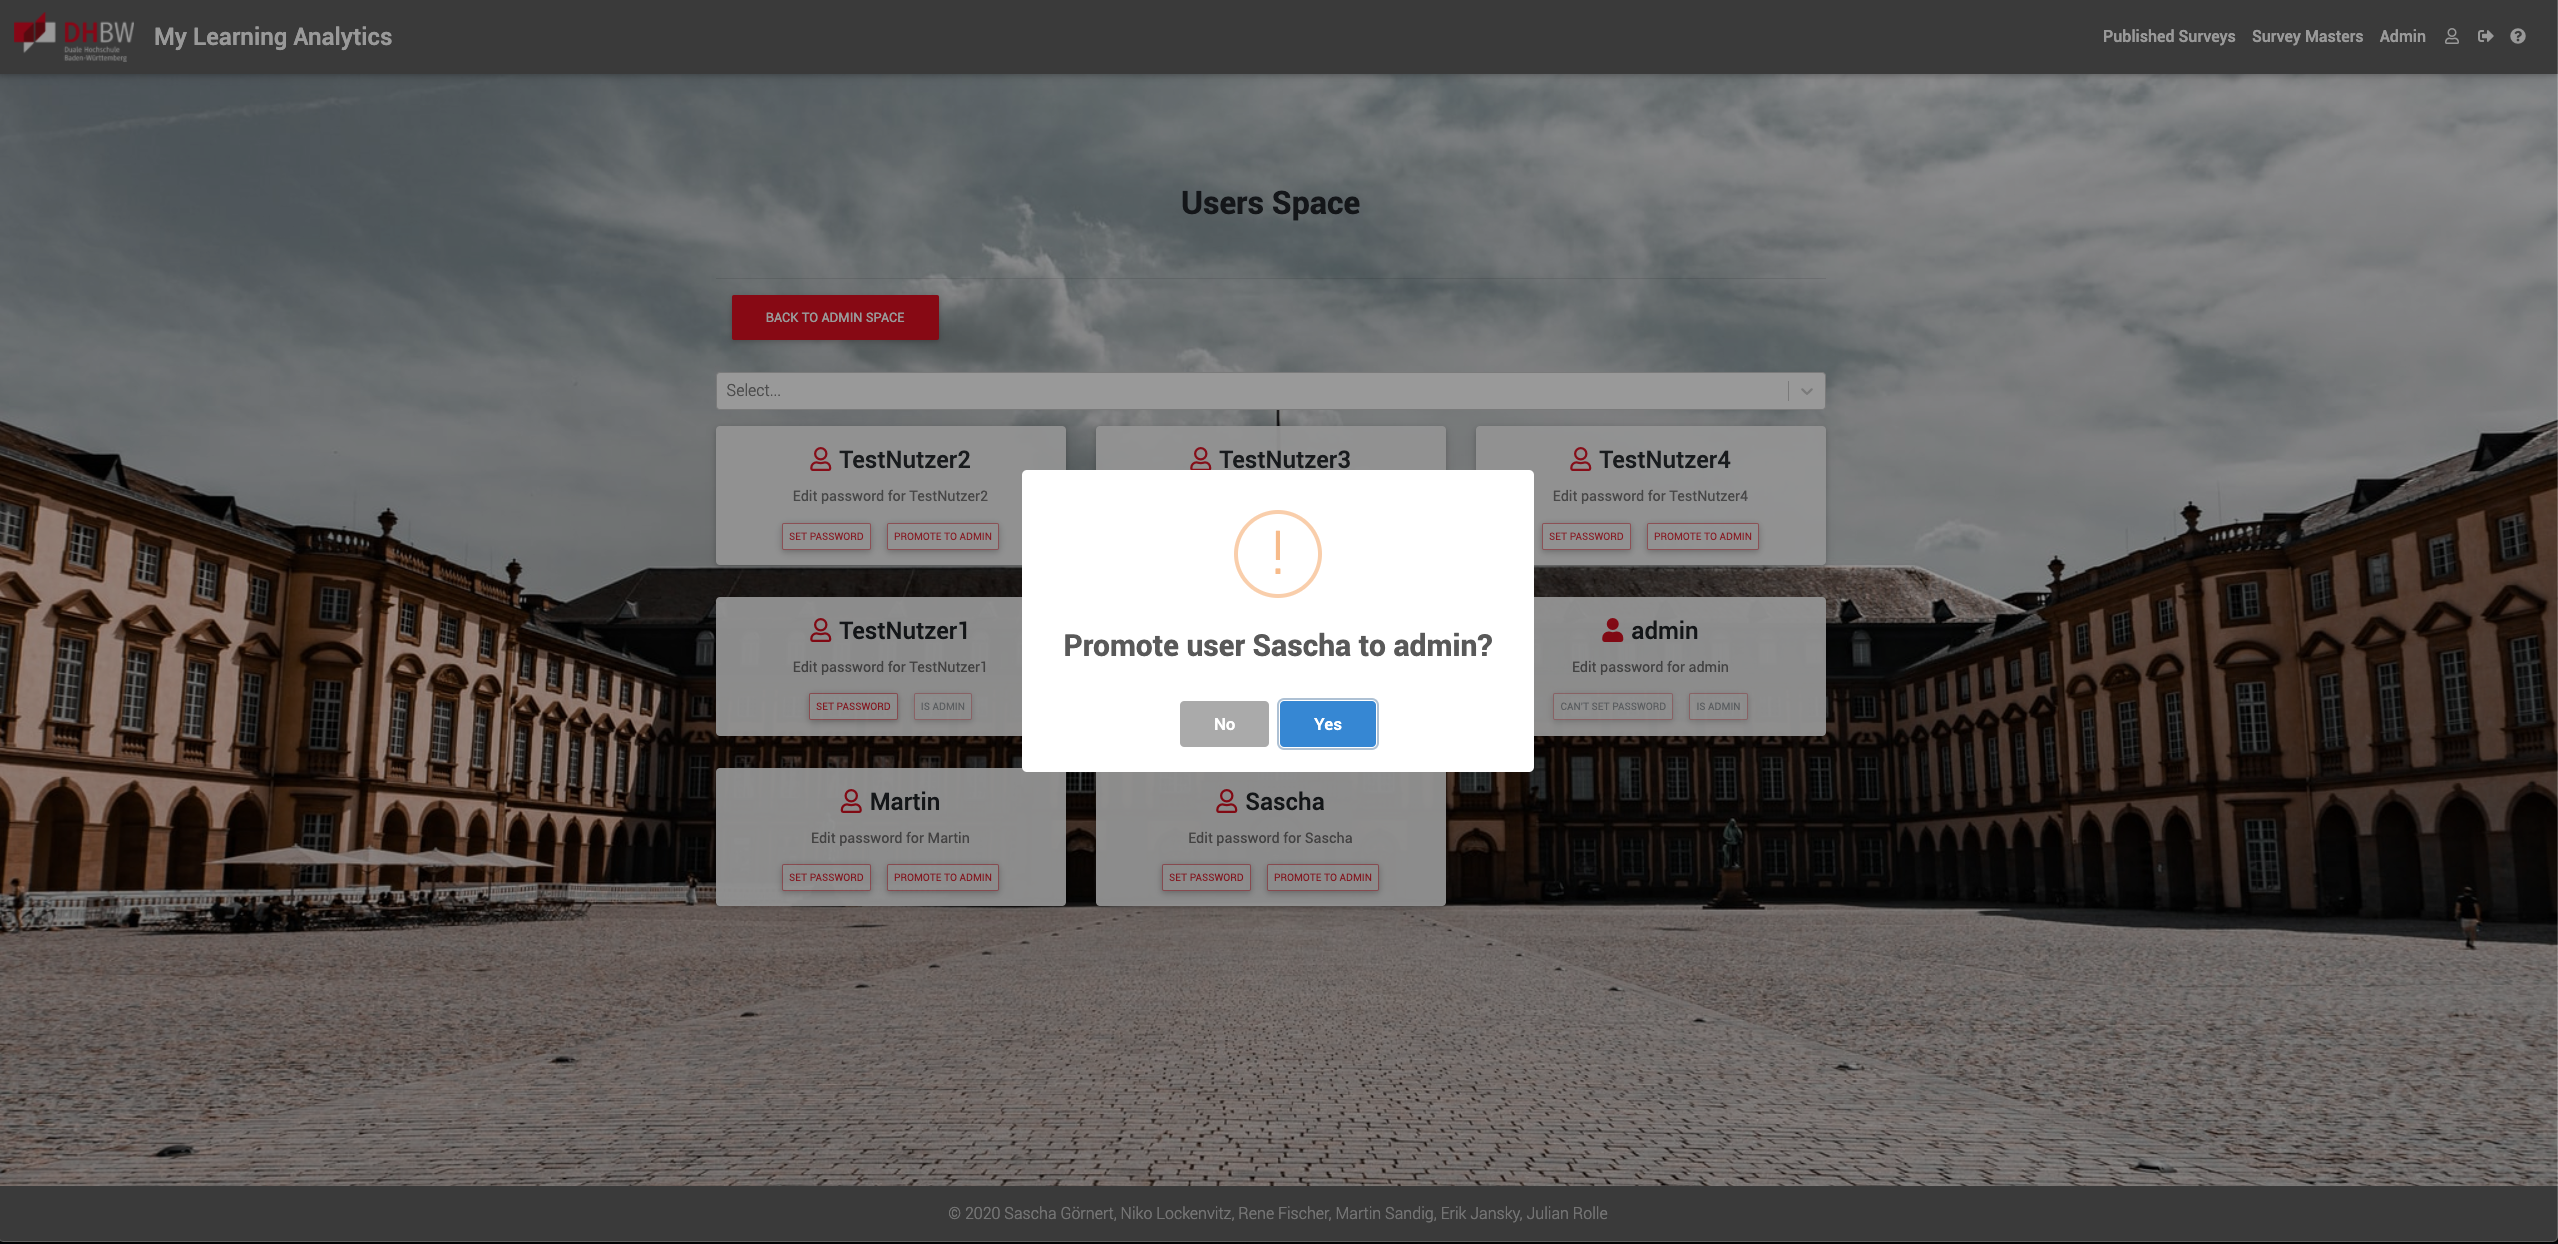
\includegraphics[width=0.95\textwidth, keepaspectratio]{img/client/AdminPromoteToAdmin.png}
	\captionsetup{justification=centering, format=plain}
	\caption[\acl{UI}: Administrator-Ernennung]{\acl{UI}: Administrator-Ernennung \\ \quelleScreenshot}
	\label{fig:AdminPromoteToAdminImplement}
\end{figure}
